\documentclass[12pt,a4paper]{jsarticle}
\usepackage[dvipdfmx]{graphicx}
\usepackage[dvipdfmx]{color}
\usepackage{listings}
% to use japanese correctly, install jlistings.
\lstset{
  basicstyle={\small\ttfamily},
  identifierstyle={\small},
  commentstyle={\small\itshape\color{red}},
  keywordstyle={\small\bfseries\color{cyan}},
  ndkeywordstyle={\small},
  stringstyle={\small\color{blue}},
  frame={tb},
  breaklines=true,
  numbers=left,
  numberstyle={\scriptsize},
  stepnumber=1,
  numbersep=1zw,
  xrightmargin=0zw,
  xleftmargin=3zw,
  lineskip=-0.5ex
}
\lstdefinestyle{customCsh}{
  language={csh},
  numbers=none,
}
\lstdefinestyle{customRuby}{
  language={ruby},
  numbers=left,
}
\lstdefinestyle{customTex}{
  language={tex},
  numbers=none,
}
\lstdefinestyle{customJava}{
  language={java},
  numbers=left,
}
\begin{document}
\title{卒業論文\\
\vspace{4cm} hikiutilsを用いた\\卒業論文作成}
\author{ 関西学院大学 理工学部 情報科学科\\\\1234 西谷滋人}
\date{\vspace{3cm} 2017年  3月\\
\vspace{3cm} 指導教員  西谷 滋人 教授}
\maketitle
\setcounter{tocdepth}{6}
\tableofcontents

\tableofcontents
\section{ユーザメモとwikiを連携するシステムの開発}
\subsection{関西学院大学 理工学部 情報科学科 3550 西谷研究室 江本沙紀}
\subsection{開発の背景}
\begin{itemize}
\item \verb|introduction(my_help2hiki_saki_introduction)|
\end{itemize}
\subsection{関連するシステムについて}
\section{関連するソフトの振る舞い}
本章では,対象とするソフトはあまり一般に普及しているものではないため,
最初にソフト(my\_helpおよびhiki)の特徴と簡単な振る舞いを紹介する.

\subsection{my\_help}
my\_helpは西谷研究室で使用しているユーザ独自のメモを作成するgemである.

gemは正式名称をRubyGemsといい,
Ruby用のライブラリを使う時に必要となるソフトウェアのことである\cite{c}.
パッケージ管理ツールgemがあることで,Ruby用ライブラリの
インストール,アンインストール,バージョン管理などを簡単に
行うことができる.
プログラミング言語Rubyのファイルに付属されていて,
無料で利用することができる.

gemの利点は次の通りである。
\begin{itemize}
\item 標準化された構造があるので,初めてみた人でも分かるようになっている.
\item gemがあることで,簡単にRuby用ライブラリをインストールでき,初心者でもアプリ機能を装備できる.
\item 誰でも作成,配布が可能である.
\end{itemize}

my\_helpが提供するコマンドとその振る舞いをhelp表示から示す.
\begin{quote}\begin{verbatim}
Usage: my_help [options]
    -v, --version                    show program Version.
    -l, --list                       list specific helps
    -e, --edit NAME                  edit NAME help(eg test_help)
    -i, --init NAME                  initialize NAME help(eg test_help).
    -m, --make                       make executables for all helps.
    -c, --clean                      clean up exe dir.
        --install_local              install local after edit helps
        --delete NAME                delete NAME help
        --hiki                       my_help2hiki
\end{verbatim}\end{quote}

my\_helpではhelpの要素をこのhelp表示と同じ構造,項目と対応する記述で表示される.
それぞれの項目はまとまりをつくり,それを-lでリスト表示される.
--versionおよび--listはgem標準に準拠するために用意されている.
上記コマンドのhelp表示のNAMEには作成したhelpの名前が入る.
--edit NAMEにより,NAMEの内容を記述し更新する,--init NAMEにより,NAMEを初期化する.
exeのディレクトリを空にするには--cleanのコマンドで実行ができる.
helpを書いた後にmy\_helpによって記述や閲覧ができるようにするために,
--install\_localが用意されている.
NAMEのhelpを消したいときには,--delete NAMEによって消去ができる.
--hikiコマンドにより,my\_helpからhikiへの自動変換を行い,wikiでブラウザ表示を行う.
my\_helpを研究室内で利用する利点は次の通りである.
\begin{itemize}
\item 研究室内でのメモの書き方が統一できる.
\item どこにメモをしたか忘れることがない.
\item 普段研究の為に使うターミナルから離れること無くメモを残すことができるので,書きたいときにすぐに書くことができる.
\end{itemize}

\subsection{hiki}
hikiとは,Rubyで書かれた高機能・高速Wikiクローンである\cite{d}.
CGI(Commond Gateway Interface)を利用して,Webサーバと連動して動く\cite{e}.
西谷研究室では,hikiの形式を利用してサイトを作り,
研究室内での情報共有やgemの使い方などを掲載して閲覧できるようにしている.
また,卒業論文の作成もhikiの形式で作成している.
hikiの特徴として次のことが挙げられる.
\begin{itemize}
\item オリジナルWikiに似たシンプルな書式を持つ.
\item プラグインによる機能拡張ができる\cite{f}.
\item 携帯からアクセスが可能.
\item アクセス制限ができる.
\item 柔軟性が高く,手軽に始められて操作が簡単\cite{g}.
\item 閲覧者でも修正,ページの追加などの編集が行える.
\item 作成したページを自動で整理する\cite{h}.
\end{itemize}
これらの特徴から,複数の人が同じ情報をリアルタイムで共有し,編集しやすいという利点を持つ.
まとめサイトを作るのに適しているとして,多くのサイトに使われている.
代表的なものに百科事典であるWikipediaがある.
本研究で作成を行う西谷研究室の内部サイトも,各研究室内メンバーのメモ(暗黙知を形式知化したもの)のまとめサイトであり,
hikiを本研究に利用することは最適であるといえる.

\paragraph{hikiとは}
Rubyで書かれた高機能・高速Wikiクローン.
参考文献3(\verb|http://hikiwiki.org/ja/| 1/27)
CGI(Commond Gateway Interface)を利用して,Webサーバと連動して動く.
参考文献4(\verb|https://ja.wikipedia.org/wiki/Hiki| 1/27)
西谷研究室では,hikiの形式を利用してサイトを作り,
研究室内での情報共有やgemの使い方などを掲載して閲覧できるようにしている.
また,卒業論文の作成にもhikiの形式で作成している.


\subsubsection{TeXとは}
「テック」または「テフ」と読む,組版ソフト.
スタンフォード大学のDonald E.Knuth教授によって作られた.
他のソフトと組み合わせて,組版結果を画面や紙に出力したり,
PDF形式で出力したりする.

\subsubsection{TeXの特徴}
\begin{itemize}
\item フリーソフトなので無料で入手でき,自由に中身を調べたり改良したりできる.
\item 商品利用が自由.
\item Windows,Mac,LinuxなどのOSに関わらず同じ動作をする.
\item TeXの文書はテキストファイルなので,普通のテキストエディタで読み書きでき,再利用やデータベース化が容易.
\item 数式の組版に定評があり,数式をテキスト形式で表す標準となっている.
\end{itemize}
\subsubsection{latexとは}
「ラテック」または「ラテフ」と読む.
DEC(現在のHP)のコンピュータ科学者Leslie Lamportによって機能強化されたTeX.
もとのTeXと同様にフリーソフトとして配布されている.

参考文献5「LATEX2e 美文書作成入門」,奥村晴彦/黒木祐介著,技術評論社,2016,p.1-3


\paragraph{gem中のhikisからhikiへの自動変換}
rubyのライブラリーパッケージの標準となるgemのdirectory構造にhikisというdirectoryを作って文書作成している.hiki --initializeでこのなかのhikidocファイルをウェブ上のhikiと同期する機能を提供する.
これによって,gem/hikisで作成した文書は,githubあるいはrubygems.orgを通じて共有可能となる.
以下にこの同期をスムーズに行うための幾つかのconventionを使用法とともにまとめている.

\paragraph{使用法,コマンド}
\begin{itemize}
\item hiki --initializeで必要なファイル(Rakefile, ./.hikirc, hiki\_help.yml)がcopyされる
\item hiki\_help.ymlは適宜~/.my\_helpにcopyしてhiki\_helpとして利用\verb|my_help参照(MyHelp_install)|
\item rake syncによってhikiディレクトリーと同期が取られる
\item rake convert 20 TARGET.pngによって,figs/TAERGET.pngに20%縮小して保存される
\item hiki -u TARGETによってブラウザー表示される
\end{itemize}
\paragraph{同期に関する制約}
\begin{itemize}
\item hikiはフラットなdirectory構造を取っている
\item hikiの文書はスネーク表記(例えば,latex2hiki\_saki)で階層構造に似せている
\item hikiのurlの接頭語となる名前をbasenameのdirectory名とする.
\item directory名が'hikis'である場合はその親directory名となる.
\item ~/.hikircのtarget directoryを同期先のdirectoryとする.
\item ~/.hikircがない場合は同期先のdirectoryを聞く.
\item それらは./.hikircに保存される
\end{itemize}
\paragraph{テキスト}
\begin{itemize}
\item テキストの拡張子は'.hiki'としている
\item hikiでのurlはテキスト前とディレクトリーから自動生成される
\item 例えば,hiki2latex\_saki/introduciton.hikiとするとhiki2latex\_saki\_introducitonと変換される
\item attach\_anchorでは
\end{itemize}\begin{quote}\begin{verbatim}
'{{attach_anchor(test.png, hiki2latex_saki)}}'
\end{verbatim}\end{quote}
と,directory指定しなければならない.


\subsection{メモ,wiki,latexの自動変換システム}
\section{方法}


\subsection{使用法,コマンド}
my\_helpからhikiに変換するときのコマンドと使用法は以下の通りである.
\begin{itemize}
\item TARGET --push : 作成したメモ(TARGET)をサーバに送る
\end{itemize}  
\begin{itemize}
\item my\_help --hiki : 作成したメモをhiki形式に変換し,wikiで表示できるようにする.
\end{itemize}

\subsection{TARGET --push のコードの詳述}
TARGET --pushのコードについて詳述する.
\begin{figure}[htbp]\begin{center}
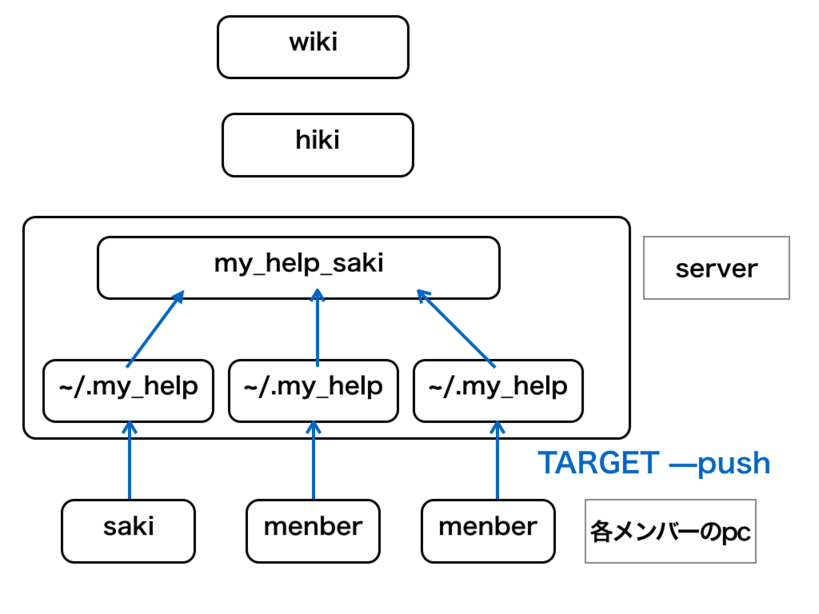
\includegraphics[width=6cm,bb=100 100 600 700]{my_help2hiki_saki.012.png}
\caption{TARGET --push}
\label{default}\end{center}\end{figure}

コードの中身は以下の通りである.
\begin{quote}\begin{verbatim}
    def push                             
      p "push my_todo"
      data_dir = File.join(ENV['HOME'],'.my_help')
      FileUtils.cd(data_dir)
      system "pwd"
      system "rm -rf ~/.my_help/*.yml~"
      system "scp -r ~/.my_help saki@nishitani0:~"
      system "ssh saki@nishitani0 ls ~/.my_help" 
    end
\end{verbatim}\end{quote}

\newpage
コードの詳細を記述する.
\begin{itemize}
\item 3,4行目
\end{itemize}
\begin{description}
\item my\_helpでは,作成したメモが.my\_helpのディレクトリに自動的に追加されるので,
ディレクトリを.my\_helpに移動する.
\end{description}
\begin{itemize}
\item 6行目
\end{itemize}
\begin{description}
\item .my\_helpにメモが追加されるとき,yaml形式のファイルで保存される.
メモを更新すると,一つ前に保存したファイルは*.yml~というファイル名
でバックアップとして残される.
\textbf{rm -rf}で不必要なファイルは削除し,サーバにコピーするときのデータ量を減らしている.
\end{description}

\begin{itemize}
\item 7行目
\end{itemize}
\begin{description}
\item
\textbf{scp -r ~/[directory名] [server名]}
のコマンドによってserverにssh接続を行い,directoryをserverにコピーする.
-rはディレクトリ全体をコピーすることを示している.
西谷研究室で利用しているnishitani0というサーバにコピーしている.
\end{description}

\begin{itemize}
\item 8行目
\end{itemize}
\begin{description}
\item nishitani0にssh接続し.my\_helpの中身を書き出して,
コピーができているかコマンドを実行した時に確認が行えるようにしている.
\end{description}

\newpage

\subsection{my\_help --hiki のコードの詳述}
my\_help --hikのコードについて詳述する.

\begin{figure}[htbp]\begin{center}
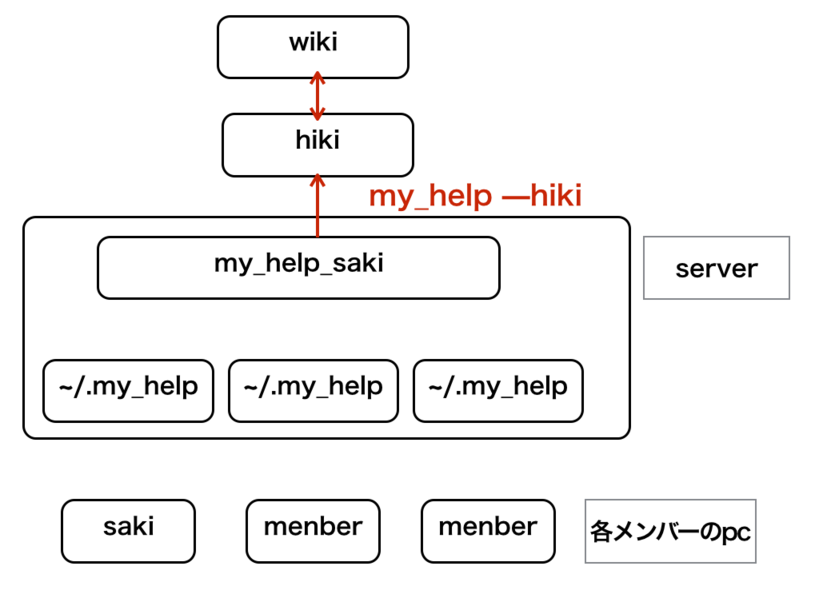
\includegraphics[width=6cm,bb=100 100 600 800]{my_help2hiki_saki.013.png}
\caption{my\_help2hiki}
\label{default}\end{center}\end{figure}

コードの中身は以下の通りである.
\begin{quote}\begin{verbatim}
  def hiki
      p 'my_help2hiki'
      system "emacs_help --to_hiki > ~/Sites/hiki-1.0/data/text/emacs_help_saki"
      system "my_todo --to_hiki > ~/Sites/hiki-1.0/data/text/my_todo_saki"
      system "ssh_help --to_hiki > ~/Sites/hiki-1.0/data/text/ssh_help_saki"
      system "open -a safari 'http://localhost/~saki/hiki-1.0/?FrontPage'"
    end
\end{verbatim}\end{quote}
\newpage
コードの詳細について記述する.
\begin{itemize}
\item 2-4行目
\end{itemize}
\begin{description}
\item my\_helpには,\textbf{TARGET --to\_hiki}というコマンドがあり,これによって
yaml形式で保存されているメモをhiki形式で書き出すことができる.
この --to\_hiki のコマンドを使ってhiki形式にしたものを,wikiで表示することのできる
フォルダである\textbf{~/Sites/hiki-1.0/data/text/}に入れることで,wikiでの表示を可能にしている.
emacs\_help,my\_todo,ssh\_helpは全て私のmy\_helpに入っているメモ.
\end{description}

\begin{itemize}
\item 5行目
\end{itemize}
\begin{description}
\item wikiのページである,図6に示したFrontPageを表示するコマンド.
これによりメモが更新されているのをすぐに確認することができる.
FrontPageは以下のようになっている.
\end{description}
\begin{quote}\begin{verbatim}
!saki's help
*[[ssh_help_saki]]
*[[my_todo_saki]]
*[[emacs_help_saki]]
\end{verbatim}\end{quote}
\begin{description}
\item 先頭に\textbf{!}をつけることで1行目のsaki's helpを見出しにし,
2~4行目は\textbf{*}によって箇条書き,角括弧でリンクになっている.
\end{description}

\begin{figure}[htbp]\begin{center}
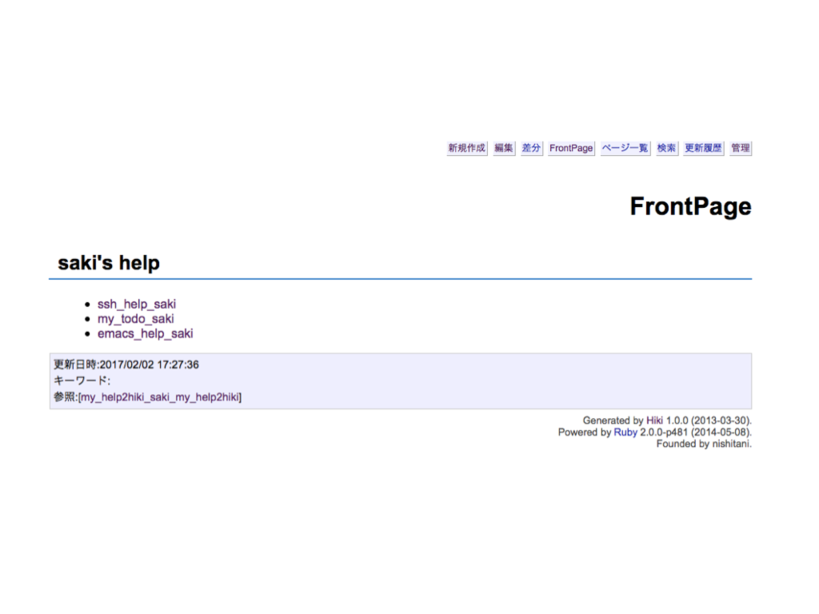
\includegraphics[clip,width=6cm,bb=100 100 600 550]{my_help2hiki_saki.002.png}
\caption{コマンドを実行したときに開くFrontPage }
\label{default}\end{center}\end{figure}


\paragraph{hiki形式で書かれた文章をlatex形式に自動変換する}
\paragraph{使用法,コマンド}
\begin{itemize}
\item hiki2latex -v : hiki2latexのversion表示
\item hiki2latex -p FILE : latexの一般的なフォーマットへ変換
\item hiki2latex -b FILE :
\end{itemize}\begin{quote}\begin{verbatim}
Usage: hiki2latex [options] FILE
    -v, --version                    show program Version.
    -l, --level VALUE                set Level for output section.
    -p, --plain FILE                 make Plain document.
    -b, --bare FILE                  make Bare document.
        --head FILE                  put headers of maketitle file.
        --pre FILE                   put preamble file.
        --post FILE                  put post file.
        --listings                   use listings.sty for preformat with style.
\end{verbatim}\end{quote}
\paragraph{gem中のhikisからhikiへの自動変換}
rubyのライブラリーパッケージの標準となるgemのdirectory構造にhikisというdirectoryを作って文書作成している.hiki --initializeでこのなかのhikidocファイルをウェブ上のhikiと同期する機能を提供する.
これによって,gem/hikisで作成した文書は,githubあるいはrubygems.orgを通じて共有可能となる.
以下にこの同期をスムーズに行うための幾つかのconventionを使用法とともにまとめている.

\paragraph{使用法,コマンド}
\begin{itemize}
\item hiki --initializeで必要なファイル(Rakefile, ./.hikirc, hiki\_help.yml)がcopyされる
\item hiki\_help.ymlは適宜~/.my\_helpにcopyしてhiki\_helpとして利用\verb|my_help参照(MyHelp_install)|
\item rake syncによってhikiディレクトリーと同期が取られる
\item rake convert 20 TARGET.pngによって,figs/TAERGET.pngに20%縮小して保存される
\item hiki -u TARGETによってブラウザー表示される
\end{itemize}
\paragraph{同期に関する制約}
\begin{itemize}
\item hikiはフラットなdirectory構造を取っている
\item hikiの文書はスネーク表記(例えば,latex2hiki\_saki)で階層構造に似せている
\item hikiのurlの接頭語となる名前をbasenameのdirectory名とする.
\item directory名が'hikis'である場合はその親directory名となる.
\item ~/.hikircのtarget directoryを同期先のdirectoryとする.
\item ~/.hikircがない場合は同期先のdirectoryを聞く.
\item それらは./.hikircに保存される
\end{itemize}
\paragraph{テキスト}
\begin{itemize}
\item テキストの拡張子は'.hiki'としている
\item hikiでのurlはテキスト前とディレクトリーから自動生成される
\item 例えば,hiki2latex\_saki/introduciton.hikiとするとhiki2latex\_saki\_introducitonと変換される
\item attach\_anchorでは
\end{itemize}\begin{quote}\begin{verbatim}
'{{attach_anchor(test.png, hiki2latex_saki)}}'
\end{verbatim}\end{quote}
と,directory指定しなければならない.

my\_help2hiki\_saki\_hiki\_syncのコピー
書き換えていく


\include{my_help_hiki_latex}
\end{document}
